\documentclass{article}

% NeurIPS 2026 preprint style (sty copied from Templates; Templates remain read-only).
% Compiler target: Overleaf pdfLaTeX (local TeX may be absent).
\usepackage[preprint]{neurips_2026}

\usepackage[utf8]{inputenc}
\usepackage[T1]{fontenc}
\usepackage{hyperref}
\usepackage{url}
\usepackage{booktabs}
\usepackage{amsfonts}
\usepackage{nicefrac}
\usepackage{microtype}
\usepackage{xcolor}
\usepackage{graphicx}

% AUTO-GENERATED headline macros (Paper Data Pipeline). Do not edit macros.tex by hand.
% AUTO-GENERATED by research_os/paper/scripts/emit_latex_from_canonical.py
% Do not edit by hand. Re-run pipeline after rebuild_canonical.
% frozen_at_utc: 2026-09-04T02:02:16.879373+00:00
% git_head: cc8cb5c60177047e910304c48fb965f6a92816ea

\newcommand{\ErrPlain}{9.68}
\newcommand{\ErrResNet}{8.41}
\newcommand{\ErrPreAct}{9.47}
\newcommand{\ErrAblationA}{8.32}
\newcommand{\AblationBStatus}{failed\_numerical\_instability}
\newcommand{\ResidualAdvantagePP}{1.27}
\newcommand{\DeltaPlainMinusResNet}{1.27}
\newcommand{\DeltaResNetMinusPlain}{-1.27}
\newcommand{\DeltaPreActMinusResNet}{1.06}
\newcommand{\DeltaAblationAMinusResNet}{-0.09}
\newcommand{\DeltaAblationAMinusPreAct}{-1.15}
\newcommand{\DeltaPreActVsResNet}{1.06}
\newcommand{\DeltaAblationAVsPreAct}{1.15}
\newcommand{\PaperResNetRef}{8.75}
\newcommand{\RepoPlainRef}{9.26}
\newcommand{\RepoResNetRef}{8.64}
\newcommand{\ReproStatus}{partially\_reproduced}
\newcommand{\ReproTolerancePP}{1.00}


\graphicspath{{figures/}}

\title{Revisiting Pre-activation Residual Blocks under a Frozen Training Recipe}
\author{
  Anonymous Author(s)\\
  Affiliation withheld pending final authorship decision\\
  \texttt{anonymous@example.com}
}

\begin{document}

\maketitle

\begin{abstract}
Residual networks remain a central architecture family for deep visual recognition, but the
effect of residual-block modifications is best interpreted together with the training recipe
under which they are evaluated.
We study a controlled question on CIFAR-10 at depth~20 with shortcut Option~A: under a frozen
post-activation ResNet-20-A training recipe, does replacing the residual block by a full
pre-activation unit reduce best test error?
We compare Plain-20, ResNet-20-A, PreAct-ResNet-20-A, and targeted BN+ReLU ablations~A/B in a
single-seed, fixed-protocol architecture comparison.
ResNet-20-A improves over Plain-20 ($\ErrResNet\%$ vs.\ $\ErrPlain\%$ best test error;
$\ResidualAdvantagePP$\,pp).
Full PreAct-ResNet-20-A reaches $\ErrPreAct\%$
($\DeltaPreActMinusResNet$\,pp higher error than ResNet-20-A);
\textbf{the hypothesized improvement was not supported under the frozen training recipe and
single-seed setting.}
Ablation~A ($\ErrAblationA\%$) improves on complete PreAct by $\DeltaAblationAVsPreAct$\,pp in
magnitude, but differs from ResNet-20-A by only $\DeltaAblationAMinusResNet$\,pp---a small
single-run gap that we do not treat as a validated improvement.
Ablation~B fails with numerical instability (\AblationBStatus) and is not used as an accuracy
baseline.
These findings do not claim that pre-activation residual units are generally ineffective; they
provide an artifact-backed, protocol-controlled negative result that narrows the hypothesis space
and motivates evaluating architecture changes jointly with optimization settings.
\end{abstract}

\section{Introduction}
\label{sec:intro}

% NeurIPS-style opening. Aligns with Conclusion claims C1--scope; macros only for headlines.
% Citations: He2016DeepResidual, He2016IdentityMappings (verified in references.bib).
% No mechanistic ``why PreAct failed'' discussion (deferred to Section~\ref{sec:discussion}).
% No new experiments; no unverified literature.

Residual networks are a central architecture family for deep visual recognition:
identity shortcuts reformulate stacked layers as residual functions and are widely used to
train deeper convolutional models~\citep{He2016DeepResidual}.
Follow-on work further revisits residual-unit design---notably pre-activation
layouts---arguing that block structure can affect optimization and
generalization~\citep{He2016IdentityMappings}.
At the same time, the practical effect of an architecture modification is not fully
separable from the training recipe under which it is evaluated: dataset protocol,
depth, shortcut option, optimizer, and schedule jointly define the comparison.

This paper studies a narrowly scoped controlled question rather than a universal ranking of
architectures.
On CIFAR-10, at depth~20 with shortcut Option~A, and under a \emph{frozen} training recipe
matched to a post-activation ResNet-20-A baseline, does replacing the post-activation residual
block by a full pre-activation residual block reduce best test error?
We do \emph{not} ask for a global ranking of pre-activation residual networks versus ResNets,
nor which family is preferable across datasets, depths, or retuned schedules.

Our experimental path is deliberately incremental and fixed-protocol.
We first compare Plain-20 (no residual shortcut) to ResNet-20-A to establish residual learning
under the shared CIFAR-10 recipe; we then evaluate PreAct-ResNet-20-A as a drop-in residual-unit
replacement; finally, we run targeted ablations A/B that remove successive BN+ReLU stages of
the pre-activation unit (Sections~\ref{sec:method}--\ref{sec:setup}).
Dataset, depth, Option~A, and the baseline training recipe remain frozen across the
improvement and ablation comparisons.
All headline runs are single-seed, which limits statistical strength
(Section~\ref{sec:limitations}).

Under this protocol, ResNet-20-A improves over Plain-20
($\ErrResNet\%$ vs.\ $\ErrPlain\%$ best test error; $\ResidualAdvantagePP$\,pp).
Full PreAct-ResNet-20-A reaches $\ErrPreAct\%$
($\DeltaPreActMinusResNet$\,pp higher error than ResNet-20-A):
\textbf{the hypothesized improvement was not supported under the frozen training recipe and
single-seed setting.}
Ablation~A attains $\ErrAblationA\%$, better than complete PreAct by
$\DeltaAblationAVsPreAct$\,pp in magnitude, yet only
$\DeltaAblationAMinusResNet$\,pp from the ResNet-20-A baseline---a small single-run gap that we
do not treat as a validated improvement.
Ablation~B fails with numerical instability (\AblationBStatus) and is not used as an accuracy
baseline.
These observations do not establish that pre-activation residual units are generally inferior
outside this recipe and scope.

\textbf{Contributions.}
We provide (i)~an artifact-backed, protocol-controlled comparison of Plain-20, ResNet-20-A, and
PreAct-ResNet-20-A under one frozen CIFAR-10 depth-20 Option~A recipe (single-run artifacts);
(ii)~an empirical negative result for the drop-in PreAct improvement hypothesis under that
clearly specified protocol;
(iii)~targeted BN+ReLU ablations that narrow how the negative result can be interpreted; and
(iv)~explicit evidence boundaries and reproducibility limitations (single-seed; no retuned
PreAct schedule; no claim of proposing a new architecture family or leaderboard-topping
accuracy).
% End Introduction.

\section{Related Work}
\label{sec:related}

% Citation-safe Related Work.
% Verified BibTeX keys only: He2016DeepResidual, He2016IdentityMappings
% (arXiv API + Crossref DOIs; project README / paper_summary pointers).
% ResearchVault Analytical Notes: not available (Phase 2/3 waived_for_demo).
% Broader architecture--recipe literature beyond these two sources: [NEEDS_VERIFICATION].
% No results from this study; no invented citations.

\subsection{Residual Learning}
\label{sec:rw-residual}

Residual learning reformulates stacked layers as learning residual functions with respect
to layer inputs, rather than unreferenced mappings~\citep{He2016DeepResidual}.
Empirically, networks with identity shortcuts are reported to be easier to optimize than
plain counterparts of comparable depth, and residual nets are evaluated on large-scale
recognition benchmarks as well as on CIFAR-10 depth studies in the original
work~\citep{He2016DeepResidual}.
The CIFAR residual family uses a $6n{+}2$ stage layout with optional projection shortcuts
(Options~A/B); our study adopts this residual-learning framing as background, without
expanding into ImageNet-scale architectures beyond what that paper already reports.

\subsection{Pre-activation Residual Networks}
\label{sec:rw-preact}

A subsequent analysis of residual units emphasizes identity mappings on the skip path and
the role of after-addition activation in signal propagation~\citep{He2016IdentityMappings}.
That line of work motivates a \emph{pre-activation} residual unit in which batch
normalization and ReLU precede the convolutional transforms
($\mathrm{BN}{\rightarrow}\mathrm{ReLU}{\rightarrow}\mathrm{Conv}$ on the residual branch),
in contrast to the original \emph{post-activation} ordering where convolutions come first and
a nonlinearity is applied after the residual addition~\citep{He2016DeepResidual,He2016IdentityMappings}.
The pre-activation redesign is presented as improving trainability and generalization in the
settings studied by~\citet{He2016IdentityMappings}; we treat those claims as the source
hypothesis space for a controlled drop-in test, not as a literature consensus that every
post-activation CIFAR recipe must benefit from an untuned replacement.

\subsection{Architectural Variants and Training Recipes}
\label{sec:rw-recipes}

Both foundational papers introduce residual units together with concrete optimization
protocols (optimizer, schedule, data augmentation, and evaluation
settings)~\citep{He2016DeepResidual,He2016IdentityMappings}.
In particular,~\citet{He2016IdentityMappings} study how residual-block design choices
interact with forward/backward propagation and report ablation-style comparisons among unit
variants under their training setups.
This background supports reading block redesign and training procedure as coupled
experimental factors rather than as fully separable claims.
A broader survey of how later residual variants, normalizers, or modern training recipes
co-adapt with architecture is outside the verified bibliography of this draft
{[NEEDS\_VERIFICATION]}.

\subsection{Positioning of This Study}
\label{sec:rw-position}

This paper does not propose a new general-purpose network family.
It is a controlled empirical study on CIFAR-10 depth~20 with shortcut Option~A:
establish a frozen post-activation ResNet-20-A baseline under a fixed training recipe,
test a full pre-activation residual-unit replacement under that same recipe, and run
targeted ablations of the pre-activation BN+ReLU placement.
The research question and experimental boundary are therefore narrow by design---architecture
change under a frozen baseline protocol---and should not be read as a comprehensive
re-evaluation of pre-activation residual networks across datasets, depths, or retuned
schedules.
% End Related Work.

\section{Method}
\label{sec:method}

% Evidence: Models.md; models.py (BasicBlock / PreActBasicBlock / CifarResNet / CifarPreActResNet);
% experiments/configs/phase3|phase5; research_os/paper/canonical/data.json; G4-approved scope.
% Missing at write time: research_os/paper/outline.md, claim_ledger.md, citation_plan.md.

We study depth-20 CIFAR residual networks in the $6n{+}2$ family with $n{=}3$
(three stages with $k{=}(20{-}2)/6{=}3$ residual units per stage).
All residual models below use \emph{shortcut Option~A} at spatial/channel transitions:
stride-2 max-pooling on the identity path and zero-padding of new channels
(no learned $1{\times}1$ projection).
Plain networks omit the shortcut.
Unless noted, convolutional filters are $3{\times}3$.

\subsection{Baselines: Plain-20 and ResNet-20-A}
\label{sec:method-baselines}

\paragraph{Plain-20.}
A non-residual convolutional network with the same depth and stage widths as the residual counterpart,
but without identity shortcuts.
In our implementation, each basic unit follows a post-activation layout on the residual branch
without an additive skip:
$\mathrm{Conv}{\rightarrow}\mathrm{BN}{\rightarrow}\mathrm{ReLU}{\rightarrow}\mathrm{Conv}{\rightarrow}\mathrm{BN}{\rightarrow}\mathrm{Add}{\rightarrow}\mathrm{ReLU}$
with the shortcut disabled (equivalently, no residual addition).
This model is the non-residual reference used to measure the benefit of residual learning
at depth~20.

\paragraph{ResNet-20-A (frozen control).}
The primary baseline replaces the plain unit with a post-activation residual block
\[
\mathrm{Conv}{\rightarrow}\mathrm{BN}{\rightarrow}\mathrm{ReLU}{\rightarrow}\mathrm{Conv}{\rightarrow}\mathrm{BN}{\rightarrow}\mathrm{Add}{\rightarrow}\mathrm{ReLU},
\]
where $\mathrm{Add}$ merges the residual branch with an Option~A identity path, followed by ReLU.
ResNet-20-A is \emph{frozen} for all subsequent improvement and ablation runs:
later experiments reuse its training recipe and do not retrain this checkpoint as a moving target.
Under the protocol in Section~\ref{sec:setup}, its best test error is $\ErrResNet\%$
(canonical snapshot; SoT manifests/results).

\subsection{Improvement: PreAct-ResNet-20-A}
\label{sec:method-preact}

The improvement question is whether replacing the post-activation residual unit by a
pre-activation unit---while keeping dataset, optimizer, schedule, Option~A, and depth fixed---reduces
test error relative to ResNet-20-A.
The full pre-activation residual branch is
\[
\mathrm{BN}{\rightarrow}\mathrm{ReLU}{\rightarrow}\mathrm{Conv}{\rightarrow}\mathrm{BN}{\rightarrow}\mathrm{ReLU}{\rightarrow}\mathrm{Conv},
\]
followed by $\mathrm{Add}$ with the Option~A identity path and \emph{no} post-addition ReLU
(ReLU is applied at the start of the residual transform / next block entry).
Stem and classifier head are kept compatible with the baseline network; the intentional change is
the residual-block activation order.
We denote this model \textbf{PreAct-ResNet-20-A}.
Its best test error under the frozen recipe is $\ErrPreAct\%$
(canonical snapshot).

\subsection{Ablations of the pre-activation unit}
\label{sec:method-ablations}

To localize the contribution of the two $\mathrm{BN}{+}\mathrm{ReLU}$ stages inside the full PreAct unit,
we define two controlled ablations that share Option~A and the same frozen training recipe:

\paragraph{Ablation~A.}
Remove the \emph{first} $\mathrm{BN}{+}\mathrm{ReLU}$.
The residual branch becomes
$\mathrm{Conv}{\rightarrow}\mathrm{BN}{\rightarrow}\mathrm{ReLU}{\rightarrow}\mathrm{Conv}{\rightarrow}\mathrm{Add}$.
Best test error: $\ErrAblationA\%$ (canonical snapshot).

\paragraph{Ablation~B.}
Remove the \emph{second} $\mathrm{BN}{+}\mathrm{ReLU}$.
The residual branch becomes
$\mathrm{BN}{\rightarrow}\mathrm{ReLU}{\rightarrow}\mathrm{Conv}{\rightarrow}\mathrm{Conv}{\rightarrow}\mathrm{Add}$.
In our runs this configuration did not yield a comparable accuracy trajectory:
training failed with numerical instability (\AblationBStatus; no best-test-error baseline is reported).

\subsection{What is held fixed vs.\ what varies}
\label{sec:method-controls}

Across PreAct and both ablations, configs prescribe the same CIFAR-10 split, depth-20 width pattern,
Option~A rule, and the post-activation training recipe used for ResNet-20-A
(Section~\ref{sec:setup}).
The sole intentional architectural factor under study is the residual-block nonlinearity/BN placement
(full PreAct vs.\ dropping the first or second pre-activation stage).
We do not introduce attention, Squeeze-and-Excitation, Cutout, Mixup, dropout, or other
regularizers in these runs.
We do \emph{not} claim an exhaustive log-level audit that every Phase~3/5 trajectory matched the
shared recipe with zero silent augmentation drift
\texttt{[NEEDS\_VERIFICATION]}.

\section{Experimental Setup}
\label{sec:setup}

% Evidence: canonical/data.json#protocol; experiments/configs/phase2|3|5;
% experiments/results/phase4/comparison.json#protocol; train.py transforms/optimizer;
% phase2 yaml environment; paper/conclusion.md §2 (hardware).
% Missing at write time: research_os/paper/outline.md, claim_ledger.md, citation_plan.md.

\subsection{Dataset and preprocessing}
\label{sec:setup-data}

We use \textbf{CIFAR-10} with the official $50\mathrm{k}/10\mathrm{k}$ train/test split.
Training images use random crop with padding~$4$ ($\texttt{RandomCrop}(32,\texttt{padding}{=}4)$),
random horizontal flip, conversion to tensors, and per-channel normalization with
mean $(0.4914, 0.4822, 0.4465)$ and std $(0.2023, 0.1994, 0.2010)$
as implemented in the training script.
Test images use tensor conversion and the same normalization without spatial augmentation.

\subsection{Optimization and schedule}
\label{sec:setup-optim}

Unless stated otherwise, all reported models share the following frozen recipe
(canonical protocol; Phase~2--5 configs):
\begin{itemize}
  \item \textbf{Optimizer:} SGD with momentum $0.9$ and weight decay $10^{-4}$.
  \item \textbf{Learning rate:} $0.1$, decayed by $10\times$ at iteration milestones
        $32{,}000$ and $48{,}000$ (\texttt{MultiStepLR}).
  \item \textbf{Mini-batch size:} $128$.
  \item \textbf{Training length:} $160$ epochs.
\end{itemize}
Configs prescribe the same recipe for Plain-20, ResNet-20-A, PreAct-ResNet-20-A, and Ablations~A/B;
Phase~4 comparisons are read-only aggregations of existing runs (no re-training).
Runtime identity of every transform/optimizer call across Phase~3/5 logs is not exhaustively
re-audited here
\texttt{[NEEDS\_VERIFICATION]}.

\subsection{Evaluation protocol}
\label{sec:setup-eval}

The primary metric is \textbf{best test error} ($\%$).
The implementation evaluates on the test set every $4$ epochs and selects
\texttt{best.pt} by minimum test error
(matching the reference training script's checkpoint rule).
We report the best test errors
$\ErrPlain\%$ (Plain-20),
$\ErrResNet\%$ (ResNet-20-A),
$\ErrPreAct\%$ (PreAct-ResNet-20-A), and
$\ErrAblationA\%$ (Ablation~A)
from the paper canonical snapshot
(\texttt{research\_os/paper/canonical/data.json}),
which is built from
\texttt{experiments/manifests/} and \texttt{experiments/results/}.
Ablation~B is recorded as a failed run (\AblationBStatus) and is \emph{not} assigned a
comparable best-test-error number.

\subsection{Randomness and hardware}
\label{sec:setup-hw}

\paragraph{Single-seed limitation.}
No random seed is fixed in the recorded protocol ($\texttt{seed}{=}\texttt{null}$).
Each configuration is a single completed training trajectory unless noted as failed.
Therefore we do not report mean$\pm$std over seeds, and small deltas
(e.g., Ablation~A vs.\ ResNet-20-A) must not be read as statistically tested improvements.

\paragraph{Hardware and software.}
Recorded notes for the frozen baseline protocol include an
NVIDIA GeForce RTX~3050 Laptop GPU (4\,GB) and PyTorch $2.0.1{+}\mathrm{cu117}$
under conda environment \texttt{deeplearn}
(Phase~2 config / Phase~4 protocol notes; also summarized in \texttt{paper/conclusion.md}).
We do \emph{not} claim that every Phase~3/5 canonical run used identical driver/CUDA build strings;
an earlier environment note also mentions a uv/cu118 path that may differ from the conda pin
\texttt{[NEEDS\_VERIFICATION]}.

\subsection{Scope boundaries for interpretation}
\label{sec:setup-scope}

All setup claims in this section are limited to CIFAR-10, depth~20, Option~A residual models,
the frozen post-activation training recipe above, and single-run evaluation.
We do not claim a full multi-depth Table~6 reproduction suite, ImageNet results,
or recipe retuning specialized to PreAct.

\section{Results}
\label{sec:results}

% Evidence: research_os/paper/canonical/data.json; macros.tex; tables/*.tex;
% latex/figures (from paper/figures / experiments/results); paper/analysis.md; paper/conclusion.md.
% Results report observed outcomes only (What happened?). Mechanism deferred to Discussion.

All headline test-error values and signed deltas below are taken from the paper canonical
snapshot via macros (Section~\ref{sec:setup}).
Unless noted, each completed model is a \emph{single} training run with unset seed.

\subsection{Main Results}
\label{sec:results-main}

Table~\ref{tab:main-results} lists best test error, best epoch, parameter count, and run status
for Plain-20, ResNet-20-A, PreAct-ResNet-20-A, Ablation~A, and Ablation~B.
Table~\ref{tab:deltas} reports the corresponding pairwise differences in best test error
(percentage points).

\begin{table}[t]
  \caption{Main CIFAR-10 results (best test error). Numbers are from the canonical snapshot.
  Ablation~B has no comparable best test error.}
  \label{tab:main-results}
  \centering
  \small
  % AUTO-GENERATED — do not edit by hand
% Source: research_os/paper/canonical/data.json
\begin{tabular}{lrrrl}
\toprule
Model & Best test err. (\%) & Best epoch & Params & Status \\
\midrule
  Plain-20 & 9.68 & 132 & 270,410 & completed \\
  ResNet-20-A & 8.41 & 132 & 270,410 & completed \\
  PreAct-ResNet-20-A & 9.47 & 128 & 270,314 & completed \\
  Ablation-A & 8.32 & 124 & 269,738 & completed \\
  Ablation-B & N/A & --- & 269,642 & failed (numerical\_instability) \\
\bottomrule
\end{tabular}

\end{table}

\begin{table}[t]
  \caption{Pairwise differences in best test error (percentage points; canonical deltas).}
  \label{tab:deltas}
  \centering
  \small
  % AUTO-GENERATED — do not edit by hand
\begin{tabular}{lr}
\toprule
Comparison & $\Delta$ best test err. (pp) \\
\midrule
ResNet-20-A $-$ Plain-20 & -1.27 \\
PreAct $-$ ResNet-20-A & 1.06 \\
Ablation-A $-$ ResNet-20-A & -0.09 \\
Ablation-A $-$ PreAct & -1.15 \\
\bottomrule
\end{tabular}

\end{table}

Observed best test errors for completed runs:
Plain-20 $\ErrPlain\%$;
ResNet-20-A $\ErrResNet\%$;
PreAct-ResNet-20-A $\ErrPreAct\%$;
Ablation~A $\ErrAblationA\%$.
Ablation~B did not complete as a comparable accuracy run
(status \AblationBStatus).

Figure~\ref{fig:phase4-bar} summarizes best test error for the Phase~4 triad
(Plain-20 / ResNet-20-A / PreAct-ResNet-20-A).
Figure~\ref{fig:phase5-bar} includes completed Phase~5 models together with the frozen baselines.

\begin{figure}[t]
  \centering
  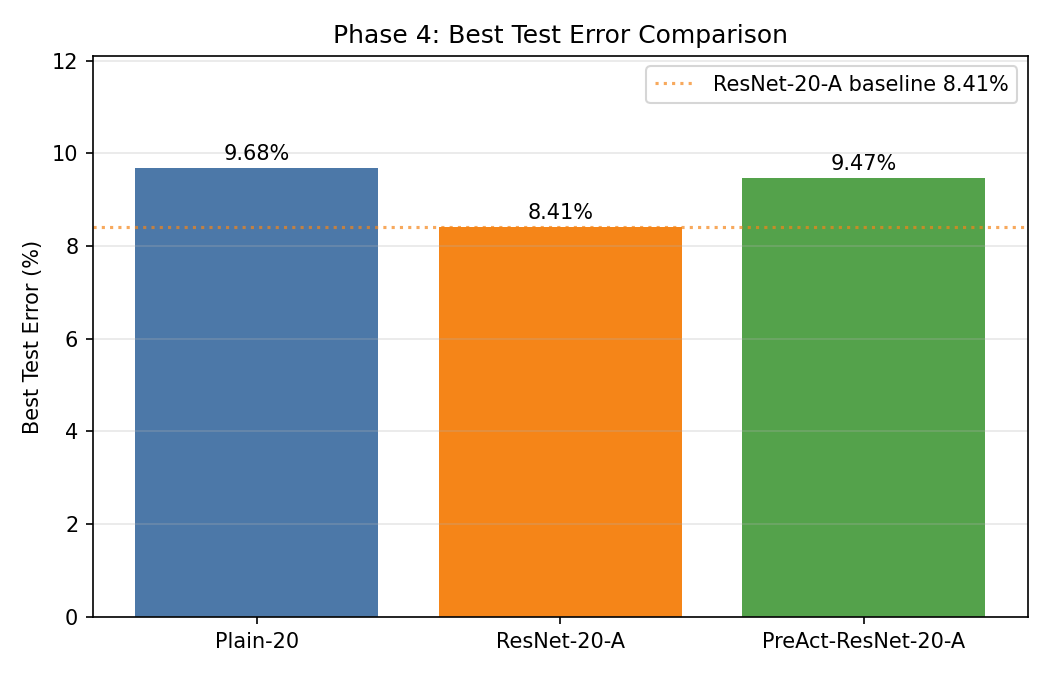
\includegraphics[width=0.82\linewidth]{phase4_best_test_error_bar.png}
  \caption{Best test error for Plain-20, ResNet-20-A, and PreAct-ResNet-20-A
  (Phase~4 comparison figure).}
  \label{fig:phase4-bar}
\end{figure}

\begin{figure}[t]
  \centering
  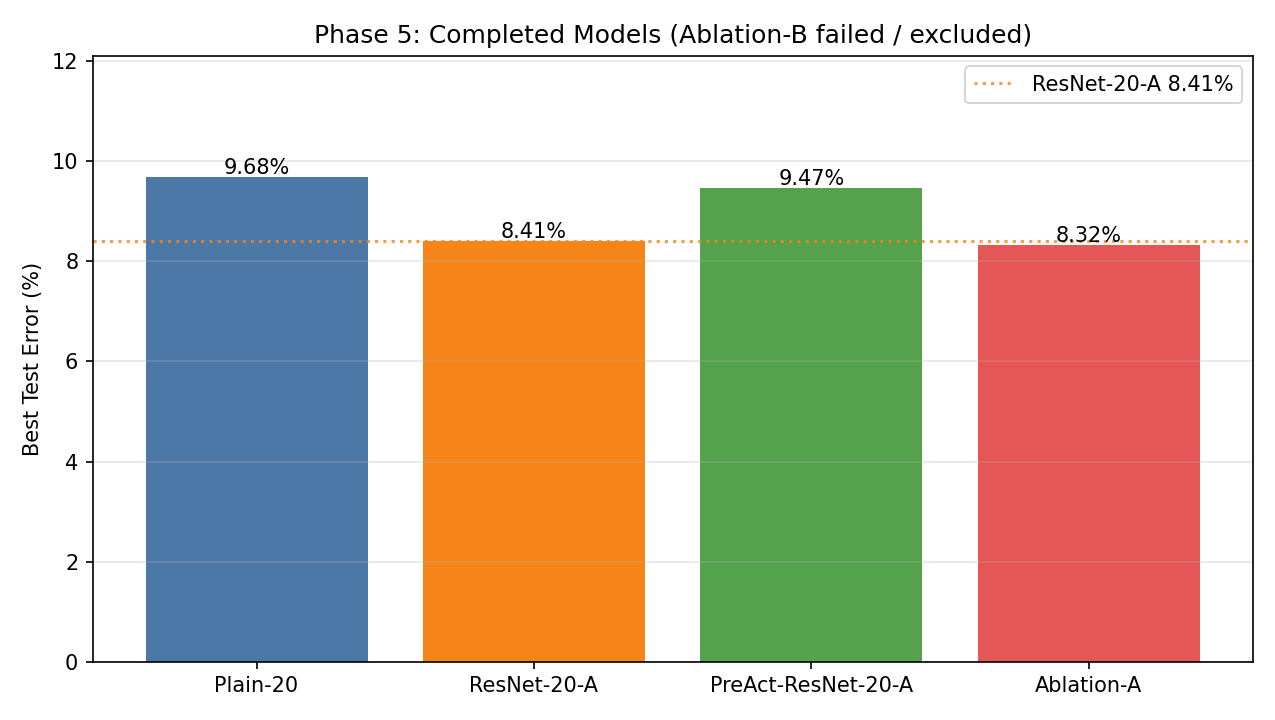
\includegraphics[width=0.82\linewidth]{phase5_best_test_error.png}
  \caption{Best test error among completed models in the Phase~5 summary figure
  (Ablation~B omitted as a failed run).}
  \label{fig:phase5-bar}
\end{figure}

\subsection{Residual Learning Comparison}
\label{sec:results-residual}

Under the shared protocol, ResNet-20-A attains best test error $\ErrResNet\%$,
while Plain-20 attains $\ErrPlain\%$.
The residual model is lower by $\ResidualAdvantagePP$ percentage points
(equivalently, ResNet-20-A $-$ Plain-20 $= \DeltaResNetMinusPlain$\,pp;
Table~\ref{tab:deltas}).

Relative to the He et~al.\ CIFAR ResNet-20 reference value $\PaperResNetRef\%$
(Table~6 in the source paper; stored as a canonical reference scalar, not a run of this project),
the observed ResNet-20-A error differs by less than the preset absolute tolerance
$\ReproTolerancePP$\,pp used in the reproduction notes
(status \ReproStatus; depth-20 subset only).

Figure~\ref{fig:phase2-plain-vs-res} shows the Phase~2 plain-vs-residual comparison plot
associated with these two completed baseline runs.

\begin{figure}[t]
  \centering
  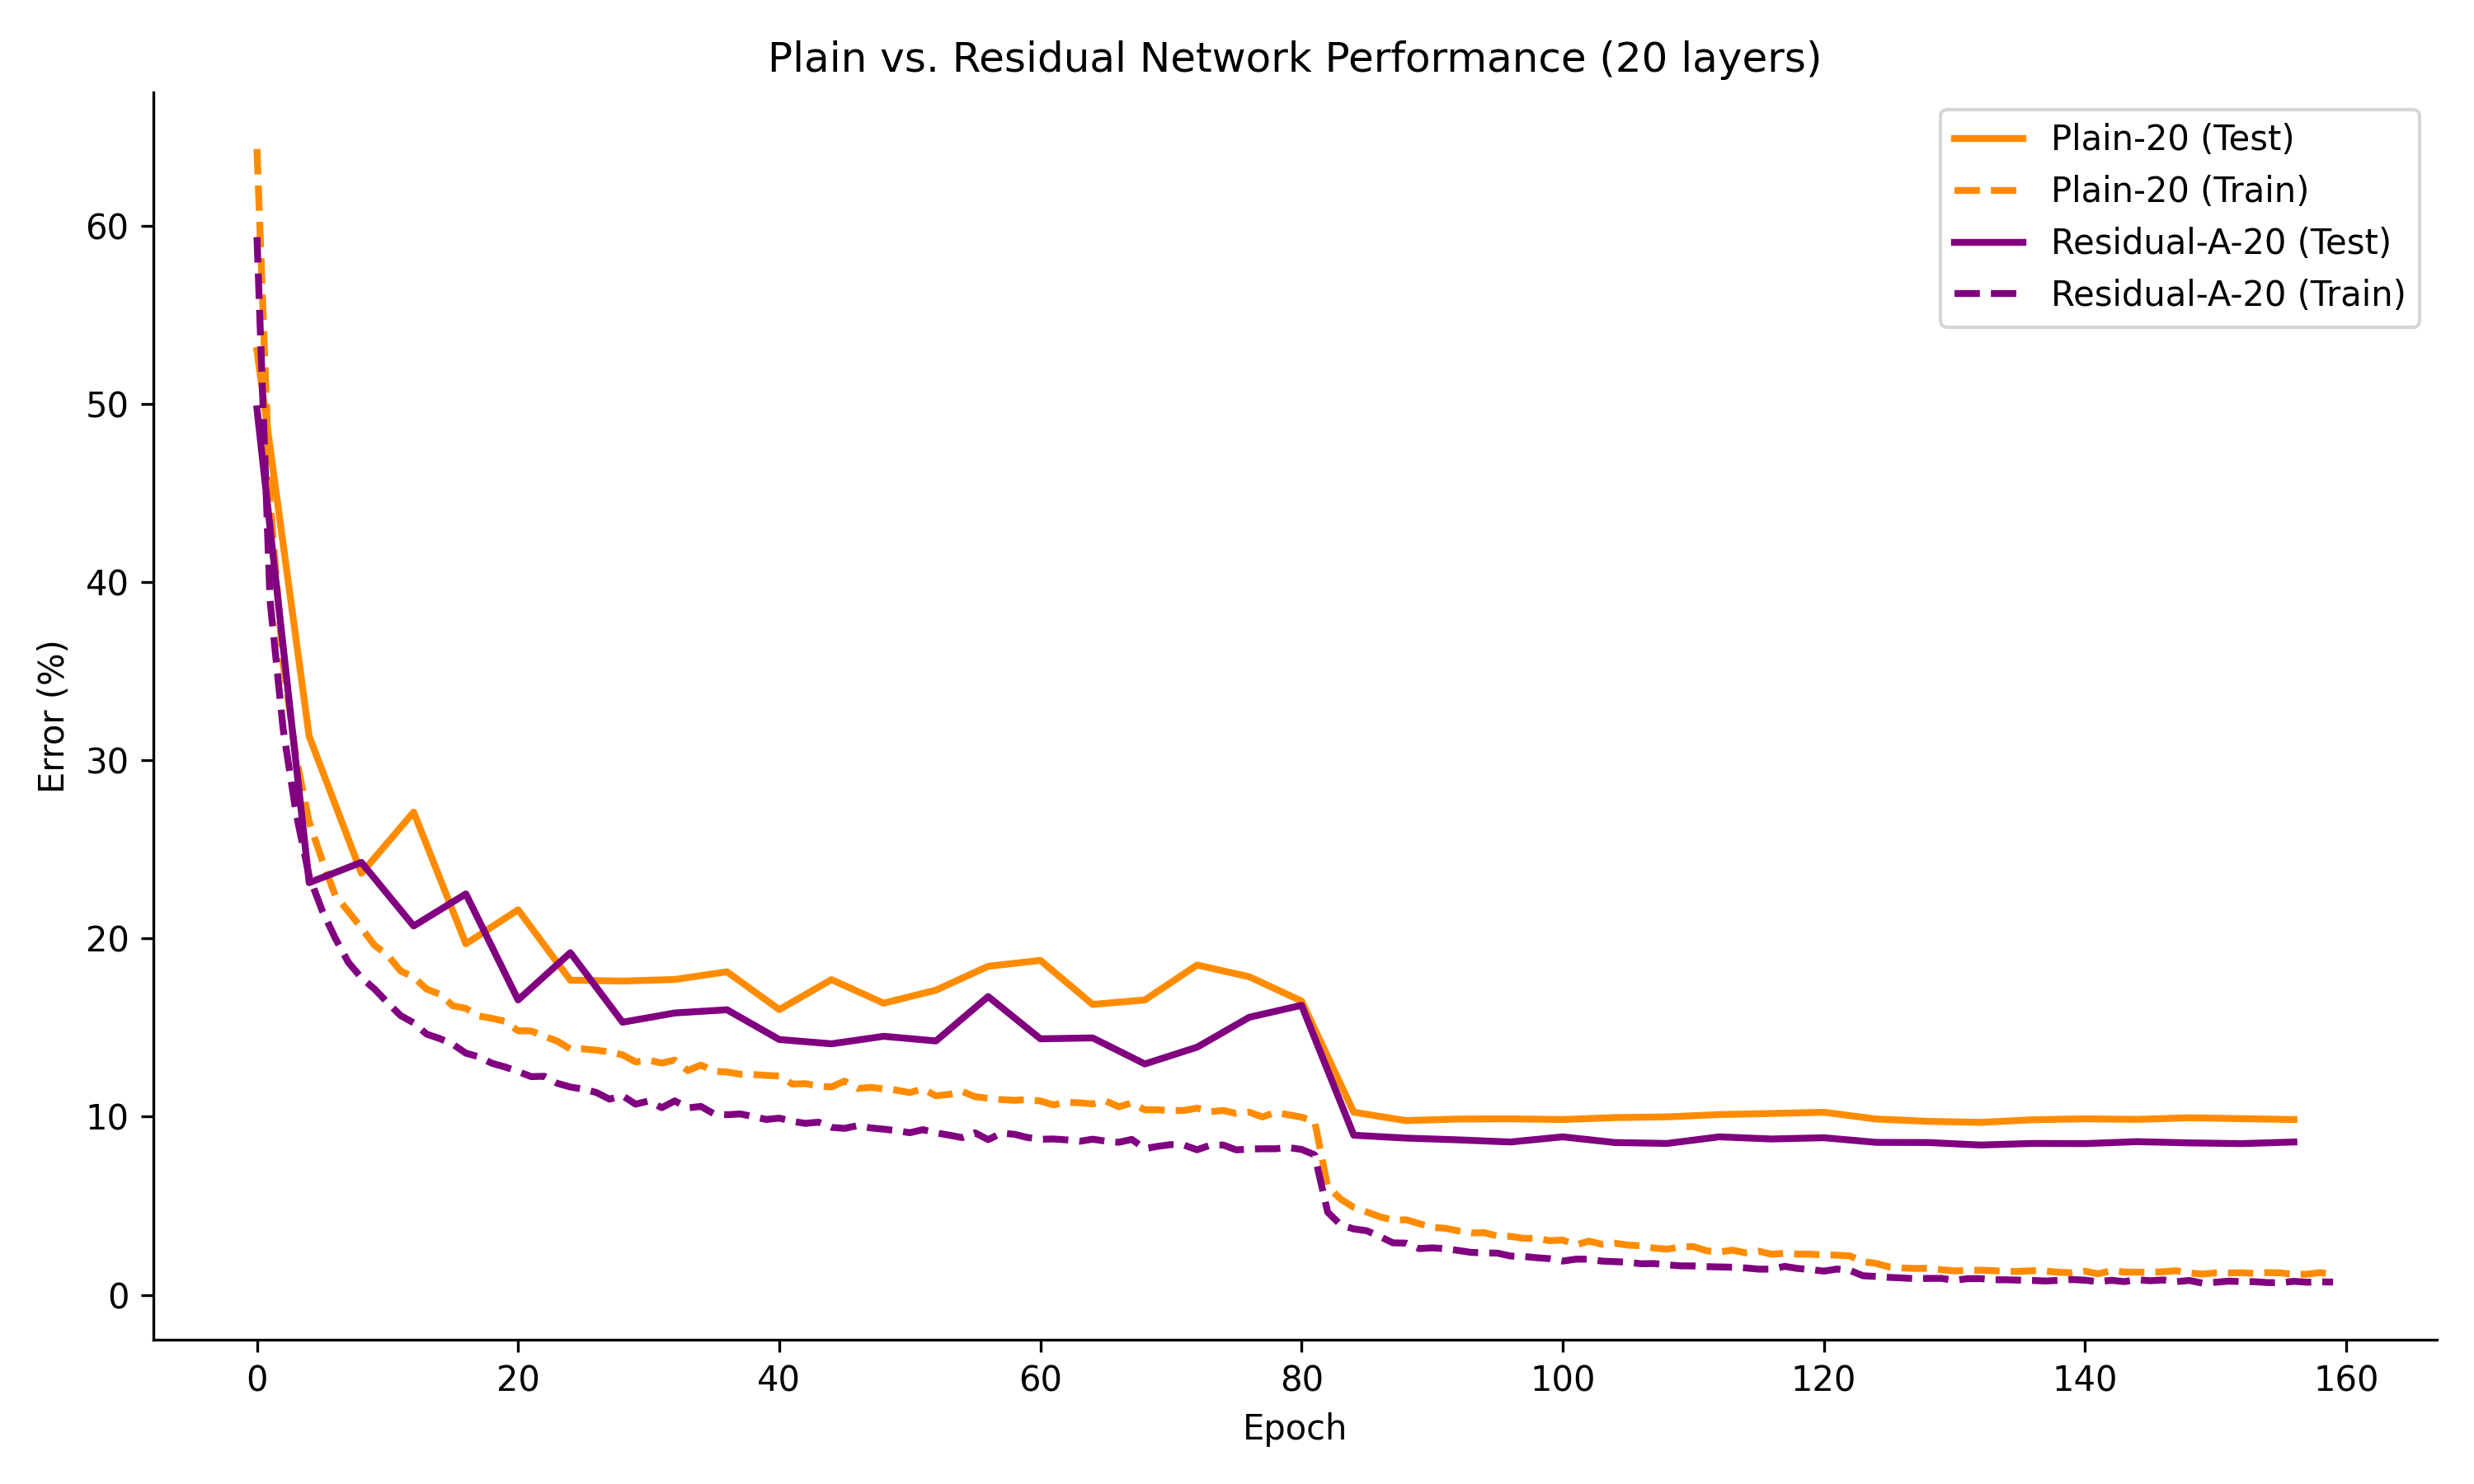
\includegraphics[width=0.82\linewidth]{phase2_plain_vs_residual.png}
  \caption{Phase~2 plain vs.\ residual comparison figure for the frozen depth-20 pair.}
  \label{fig:phase2-plain-vs-res}
\end{figure}

\subsection{Pre-activation Improvement}
\label{sec:results-preact}

With dataset, Option~A, depth, and the frozen post-activation training recipe held fixed,
replacing the residual block by the full pre-activation unit yields
PreAct-ResNet-20-A best test error $\ErrPreAct\%$.
Relative to ResNet-20-A ($\ErrResNet\%$), this is an increase of
$\DeltaPreActMinusResNet$ percentage points
(PreAct $-$ ResNet-20-A $= \DeltaPreActMinusResNet$\,pp; Table~\ref{tab:deltas}).

Thus, under this single-run frozen-recipe comparison, the pre-activation substitution
does \emph{not} reduce test error relative to the frozen ResNet-20-A control.
Figure~\ref{fig:phase4-curves} shows the corresponding Phase~4 test-error curves.

\begin{figure}[t]
  \centering
  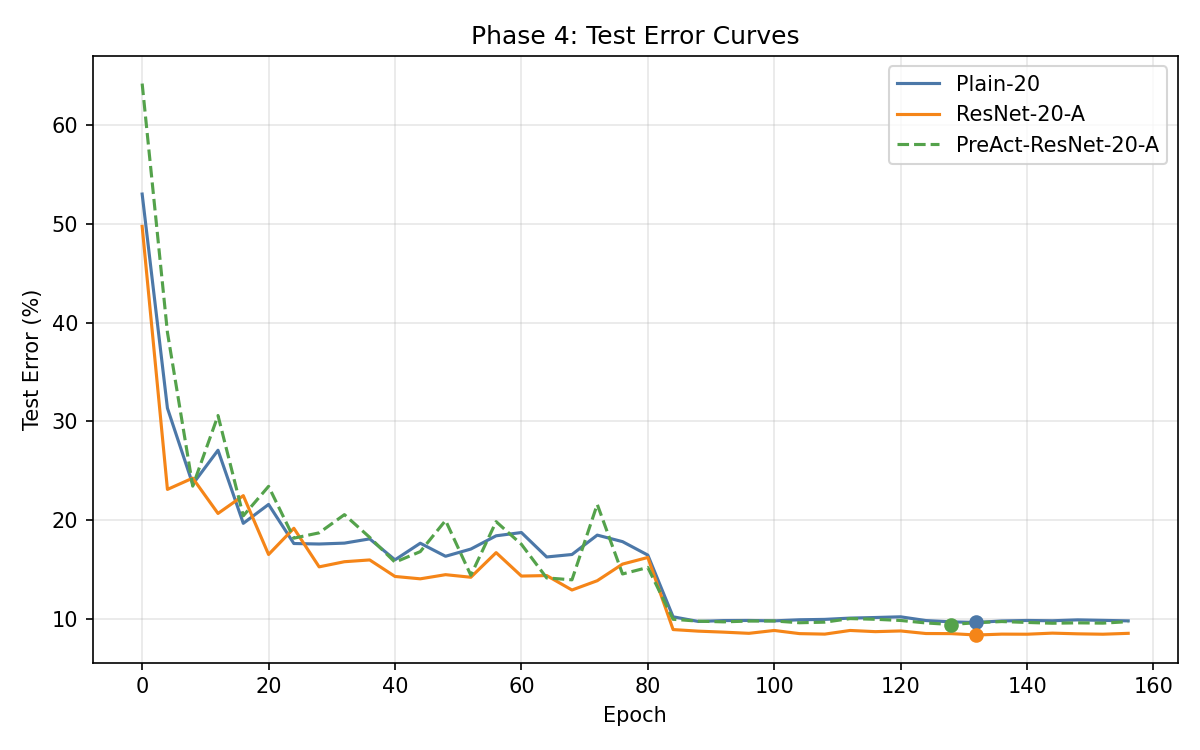
\includegraphics[width=0.82\linewidth]{phase4_test_error_curves.png}
  \caption{Phase~4 test-error curves for Plain-20, ResNet-20-A, and PreAct-ResNet-20-A.}
  \label{fig:phase4-curves}
\end{figure}

\subsection{Ablation Results}
\label{sec:results-ablation}

\paragraph{Ablation~A.}
Removing the first $\mathrm{BN}{+}\mathrm{ReLU}$ from the full PreAct unit yields
best test error $\ErrAblationA\%$.
Versus full PreAct ($\ErrPreAct\%$), Ablation~A is lower by
$\DeltaAblationAVsPreAct$ percentage points in magnitude
(Ablation~A $-$ PreAct $= \DeltaAblationAMinusPreAct$\,pp).
Versus ResNet-20-A ($\ErrResNet\%$), Ablation~A differs by
$\DeltaAblationAMinusResNet$ percentage points
(Ablation~A $-$ ResNet-20-A $= \DeltaAblationAMinusResNet$\,pp).
This latter gap is a small single-run difference and is reported as an observed delta only.

\paragraph{Ablation~B.}
Removing the second $\mathrm{BN}{+}\mathrm{ReLU}$ produced a failed training run with
numerical instability (status \AblationBStatus).
No best test error is reported for Ablation~B, and the failed trajectory is \emph{not}
used as an accuracy baseline in Table~\ref{tab:main-results} or Table~\ref{tab:deltas}.

\subsection{Summary of Observations}
\label{sec:results-summary}

Under the frozen CIFAR-10 depth-20 protocol of Section~\ref{sec:setup}, the recorded outcomes are:
\begin{enumerate}
  \item ResNet-20-A ($\ErrResNet\%$) improves on Plain-20 ($\ErrPlain\%$) by
        $\ResidualAdvantagePP$\,pp.
  \item Full PreAct-ResNet-20-A ($\ErrPreAct\%$) has higher best test error than ResNet-20-A by
        $\DeltaPreActMinusResNet$\,pp on this single run.
  \item Ablation~A ($\ErrAblationA\%$) is better than full PreAct by
        $\DeltaAblationAVsPreAct$\,pp in magnitude, and differs from ResNet-20-A by
        $\DeltaAblationAMinusResNet$\,pp.
  \item Ablation~B fails with numerical instability and contributes no comparable
        best-test-error number.
\end{enumerate}
Interpretation of mechanisms and broader generalization is deferred to the discussion.

\section{Discussion}
\label{sec:discussion}

% Evidence map: paper/analysis.md (Observed/Inferred/Speculative); paper/conclusion.md;
% canonical macros; Results (Sec.~\ref{sec:results}). No new experiments. No invented citations.

We revisit the research question under the frozen CIFAR-10 protocol of
Section~\ref{sec:setup}:
whether replacing the ResNet-20-A post-activation residual block by a full
pre-activation unit reduces best test error.
Throughout, we separate \emph{observed evidence} (what the recorded runs show),
\emph{interpretation} (what those outcomes suggest in context),
\emph{hypothesis} (plausible mechanisms that remain unproven),
and \emph{unsupported causal claims} (statements not licensed by the present design).

\subsection{What the Baseline Establishes}
\label{sec:disc-baseline}

\paragraph{Observed.}
Under the shared recipe, ResNet-20-A attains best test error $\ErrResNet\%$,
whereas Plain-20 attains $\ErrPlain\%$
(Section~\ref{sec:results-residual}; Table~\ref{tab:main-results}).
The residual model is lower by $\ResidualAdvantagePP$ percentage points
($\DeltaResNetMinusPlain$\,pp for ResNet $-$ Plain).

\paragraph{Interpretation.}
Within this depth-20, single-seed CIFAR-10 setting, the residual shortcut is associated
with a clear reduction in best test error relative to the matched plain network.
This supports treating ResNet-20-A as a usable frozen control for subsequent architecture
substitutions, rather than as an under-implemented baseline.

\paragraph{Unsupported causal claim.}
These two runs do not by themselves prove residual learning is universally beneficial
beyond the tested depth, dataset, and recipe, nor do they identify which shortcut
implementation details are necessary for the observed gap.

\subsection{Why the Pre-activation Replacement Did Not Improve the Baseline}
\label{sec:disc-preact}

\paragraph{Observed.}
Full PreAct-ResNet-20-A reaches $\ErrPreAct\%$ best test error, which is
$\DeltaPreActMinusResNet$ percentage points \emph{higher} than ResNet-20-A
(Section~\ref{sec:results-preact}).
The preset improvement hypothesis required a reduction of at least $0.30$\,pp
relative to the frozen control; that threshold was not met
(Section~\ref{sec:setup}; Phase~3 design record summarized in \texttt{paper/conclusion.md}).

\paragraph{Interpretation.}
The substitution is an architecture change that also relocates BN and ReLU relative to
convolution, while the training recipe (learning rate, milestones, epochs, augmentation,
Option~A, depth) remains the post-activation baseline recipe.
Therefore the negative outcome is evidence about
\textbf{pre-activation as a drop-in replacement under the frozen recipe},
not evidence that pre-activation is intrinsically inferior in all training regimes.

\paragraph{Hypothesis (unproven).}
A plausible account---consistent with, but not proven by, the recorded trajectories---is
that the frozen schedule is poorly matched to the PreAct unit on this shallow network,
so that the intended benefit of cleaner identity mappings does not appear as lower test error
in this single run.
\texttt{[NEEDS\_VERIFICATION]}: controlled learning-rate / schedule retuning for PreAct
was not performed in the present evidence bundle.

\paragraph{Unsupported causal claim.}
We do \emph{not} endorse blanket dismissals of pre-activation residual units
(for example, claims of intrinsic inferiority across recipes, depths, or datasets).
No multi-seed estimate, no PreAct-specific hyperparameter search, and no deeper-network
sweep are available here to support such generalizations.

\subsection{Evidence from the Ablations}
\label{sec:disc-ablation}

\paragraph{Ablation~A --- observed.}
Removing the first $\mathrm{BN}{+}\mathrm{ReLU}$ yields $\ErrAblationA\%$ best test error.
Relative to full PreAct, this is $\DeltaAblationAMinusPreAct$\,pp
(magnitude $\DeltaAblationAVsPreAct$\,pp).
Relative to ResNet-20-A, the difference is $\DeltaAblationAMinusResNet$\,pp
(Section~\ref{sec:results-ablation}).

\paragraph{Ablation~A --- interpretation.}
The large recovery versus full PreAct indicates that, in this frozen setting, the
\emph{presence of the first pre-activation stage} co-occurs with the worse PreAct outcome.
The small gap versus ResNet-20-A is an observed single-seed delta only; it does not license
claims of a statistically validated improvement over the frozen baseline.

\paragraph{Ablation~A --- hypothesis vs.\ unsupported claim.}
\emph{Hypothesis:} the first BN+ReLU may be mismatched to the shallow CIFAR-10 depth-20 network when
trained with the post-activation recipe.
\emph{Unsupported:} we have not identified a causal pathway (gradients, feature statistics,
or optimization geometry) that proves why the first stage hurts; no interventional
experiment beyond this one architectural ablation is recorded.

\paragraph{Ablation~B --- observed.}
Removing the second $\mathrm{BN}{+}\mathrm{ReLU}$ produced numerical instability
(status \AblationBStatus) and no comparable best test error
(Section~\ref{sec:results-ablation}).

\paragraph{Ablation~B --- interpretation.}
Under the current learning rate $0.1$ recipe, this configuration is not a valid accuracy
comparator. The failure constrains what can be said about ``accuracy contribution'' of the
second stage: the present evidence speaks to \emph{trainability under this recipe}, not to a
ranked test-error effect.

\paragraph{Ablation~B --- unsupported claim and future check.}
We do \emph{not} conclude that the second BN is universally indispensable for all depths,
optimizers, or learning rates.
A natural follow-up is a controlled rescue experiment (for example, lower learning rate or
warmup) to test whether Ablation~B can become trainable; such a rescue is
\texttt{[NEEDS\_VERIFICATION]} / future work and is not claimed as completed here.

\subsection{Interpretation of the Negative Result}
\label{sec:disc-negative}

\paragraph{Hypothesis status.}
The improvement hypothesis---that full PreAct would strictly reduce best test error relative
to frozen ResNet-20-A under the shared protocol---is \textbf{not supported} by the recorded
evidence ($\ErrPreAct\%$ vs.\ $\ErrResNet\%$; $+\DeltaPreActMinusResNet$\,pp).

\paragraph{Proper scope of the negative result.}
What is supported is a scoped statement:
\textbf{the hypothesized improvement was not supported under the frozen training recipe and
single-seed setting.}
What is \emph{not} supported is any blanket dismissal of pre-activation residual units
outside that scope.

\subsection{Research Implications}
\label{sec:disc-implications}

\begin{enumerate}
  \item \textbf{Architecture and recipe are coupled.}
  Evaluating a block reordering while freezing the post-activation schedule answers a
  drop-in question; it does not answer the best attainable PreAct accuracy after retuning.
  \item \textbf{Negative results shrink the hypothesis space.}
  Ruling out ``free gain from full PreAct under this recipe'' focuses follow-ups on
  recipe rescue, multi-seed estimation, and finer ablations, rather than on claiming a
  universal architectural ranking.
  \item \textbf{Next experiments should be controlled, not rhetorical.}
  Priority directions already suggested by the evidence bundle include multi-seed repeats
  for ResNet-20-A vs.\ Ablation~A, and LR/schedule rescue attempts for PreAct / Ablation~B
  (\texttt{paper/analysis.md}, \texttt{paper/conclusion.md}).
  These remain proposals until executed and registered in the experimental SoT.
\end{enumerate}

\section{Limitations}
\label{sec:limitations}

% Scope bounds on conclusions. Observed evidence in Results remains valid within these bounds.
% Evidence: canonical protocol (seed null); paper/analysis.md; paper/conclusion.md; Method/Setup/Discussion.

The observations in Sections~\ref{sec:results}--\ref{sec:discussion} remain valid as
single-run records under the frozen protocol.
The limitations below restrict the \emph{scope of conclusions}, not the existence of those
recorded outcomes.

\subsection{Single-seed Evaluation}
\label{sec:lim-seed}

All primary configurations are single training trajectories with unset seed
($\texttt{seed}{=}\texttt{null}$ in the canonical protocol; Section~\ref{sec:setup}).
We do not report mean$\pm$std over seeds, and we do not perform formal significance tests.
Consequently, small deltas must not be read as statistically validated effects.
In particular, the Ablation~A vs.\ ResNet-20-A gap of $\DeltaAblationAMinusResNet$\,pp
(Section~\ref{sec:results-ablation}) is an observed single-run difference only.

\subsection{Frozen Training Recipe}
\label{sec:lim-recipe}

PreAct-ResNet-20-A and both ablations reuse the frozen post-activation baseline recipe
(learning rate, milestones, epochs, augmentation, Option~A, depth).
No PreAct-specific learning-rate or schedule retuning is present in the evidence bundle.
The negative PreAct comparison therefore answers whether a \emph{drop-in} pre-activation
replacement improves ResNet-20-A \textbf{under the frozen recipe}
($\ErrPreAct\%$ vs.\ $\ErrResNet\%$; $\DeltaPreActMinusResNet$\,pp).
It does \emph{not} answer whether a sufficiently retuned PreAct model would outperform
ResNet-20-A.

\subsection{Limited Architecture and Dataset Scope}
\label{sec:lim-scope}

All reported runs use CIFAR-10, depth~20, and Option~A residual shortcuts within the
present residual implementation (Sections~\ref{sec:method}--\ref{sec:setup}).
We do not claim ImageNet results, multi-depth Table~6 coverage, or transfer to other
datasets or network families.
Reproduction status for the residual baseline remains \ReproStatus at the depth-20 subset
tolerance $\ReproTolerancePP$\,pp (canonical reference), not a full-suite reproduction.

\subsection{Ablation~B Failure}
\label{sec:lim-ablation-b}

Ablation~B failed with numerical instability under the current recipe
(status \AblationBStatus) and therefore has no comparable best test error
(Section~\ref{sec:results-ablation}).
This limits accuracy comparisons involving Ablation~B; it does not license a universal claim
that the second BN is necessary in all settings.
A controlled rescue experiment (for example, lower learning rate) is not part of the present
SoT
\texttt{[NEEDS\_VERIFICATION]} / future work.

\subsection{Reproducibility and Environment Scope}
\label{sec:lim-env}

The evidence is a registered set of single-run artifacts (manifests, results, and the
canonical snapshot), not a multi-seed replication study.
Hardware and software notes for the frozen baseline protocol include an
NVIDIA GeForce RTX~3050 Laptop GPU (4\,GB) and PyTorch $2.0.1{+}\mathrm{cu117}$ under
conda \texttt{deeplearn} (Section~\ref{sec:setup}).
Exact Phase~3/5 driver/CUDA string identity is not exhaustively audited in the present paper
package
\texttt{[NEEDS\_VERIFICATION]};
we do not invent additional seed, driver, or CUDA details beyond the recorded sources.

\section{Conclusion}
\label{sec:conclusion}

% Compact NeurIPS-style closing. Evidence: canonical macros; Results/Discussion/Limitations;
% paper/analysis.md; paper/conclusion.md. No new experiments. No invented citations.

We asked whether, on CIFAR-10 depth~20 with Option~A and a frozen post-activation training
recipe matched to ResNet-20-A, replacing the residual block by a full pre-activation unit
reduces best test error.
All primary comparisons are single-seed runs under that shared protocol
(Sections~\ref{sec:setup}--\ref{sec:limitations}).

First, residual learning is supported in this setting:
ResNet-20-A attains $\ErrResNet\%$ best test error versus $\ErrPlain\%$ for Plain-20
($\ResidualAdvantagePP$\,pp advantage; Section~\ref{sec:results-residual}).
Second, full PreAct-ResNet-20-A reaches $\ErrPreAct\%$, i.e.\
$\DeltaPreActMinusResNet$\,pp higher error than the frozen ResNet-20-A control;
\textbf{the hypothesized improvement was not supported under the frozen training recipe and
single-seed setting}
(Section~\ref{sec:disc-negative}).
Third, Ablation~A ($\ErrAblationA\%$) improves on full PreAct by
$\DeltaAblationAVsPreAct$\,pp in magnitude, while differing from ResNet-20-A by only
$\DeltaAblationAMinusResNet$\,pp---a small single-run gap that we do not treat as a
validated improvement.
Ablation~B fails with numerical instability (\AblationBStatus) and is not used as an
accuracy baseline.

These findings are scoped to CIFAR-10, depth~20, Option~A, the present implementation, the
frozen baseline recipe, and single-seed evaluation; they do not extend to ImageNet, deeper
networks, other datasets, retuned PreAct schedules, or multi-seed statistical conclusions.
More broadly, the study illustrates that architectural block changes should be interpreted
jointly with the optimization recipe, and that a carefully scoped negative result can shrink
the hypothesis space---motivating controlled recipe-rescue and multi-seed validation rather
than a blanket rejection of pre-activation residual units.


\bibliographystyle{plainnat}
\bibliography{references}

\end{document}
